\documentclass{article}
\usepackage{amsmath}
\usepackage{tikz}
\usetikzlibrary{arrows.meta, shapes.geometric, calc, shadows}
\tikzstyle{square} = [regular polygon,regular polygon sides=4]

\begin{document}
\section{Flooding algorithm}
For Equations
\begin{equation}
  \label{eq:cut-1}
  m_{1}x+m_{2}y+m_{3}z = \alpha
\end{equation}
Supposed it ranks as $m_{1}<m_{2}<m_{3}$.

Three intercepts on the coordcates are
\begin{equation}
  \label{eq:cut-1}
  m_{1}x+m_{2}y+m_{3}z = \alpha
\end{equation}

\begin{equation}
  \begin{aligned}
  \label{eq:cut-1}
  h_{1} = \frac{\alpha}{m_{1}} \\
  h_{2} = \frac{\alpha}{m_{2}} \\
  h_{3} = \frac{\alpha}{m_{3}}
  \end{aligned}
\end{equation}

where $h_{1} > h_{2} > h_{3}$.

Based on the 


\begin{figure}
\centering
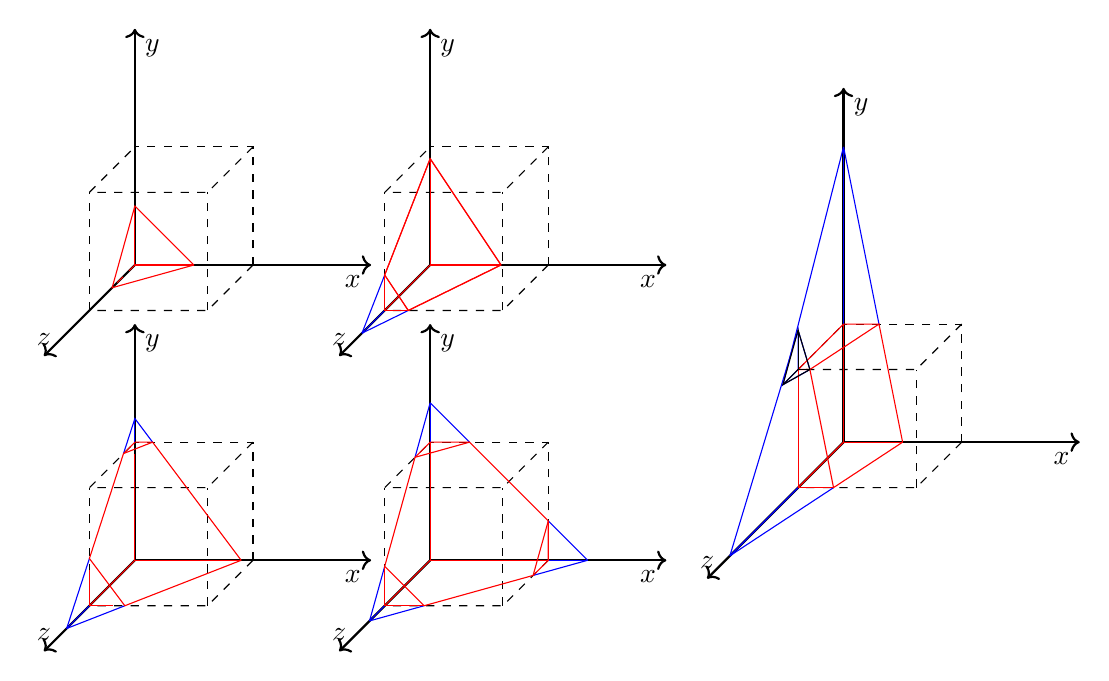
\begin{tikzpicture}[scale=1.5]

% define origin shift
\tikzstyle{shifts}=[xshift=\xo, yshift=\yo]

% cut1
\pgfmathsetmacro{\xo}{0}
\pgfmathsetmacro{\yo}{2.5cm}

\draw[shifts, thick,->] (0,0,0) -- (2,0,0) node[anchor=north east]{$x$};
\draw[shifts, thick,->] (0,0,0) -- (0,2,0) node[anchor=north west]{$y$};
\draw[shifts, thick,->] (0,0,0) -- (0,0,2) node[anchor=south]{$z$};

\draw[shifts, dashed] (1,0,0) -- (1,1,0) -- (0,1,0) ;
\draw[shifts, dashed] (1,0,0) -- (1,0,1) -- (0,0,1) ;
\draw[shifts, dashed] (1,1,0) -- (1,1,1) -- (0,1,1) -- (0,1,0) ;
\draw[shifts, dashed] (0,0,1) -- (0,1,1) ;
\draw[shifts, dashed] (1,0,1) -- (1,1,1) ;

\draw[shifts, -,red] (0.5,0,0) -- (0,0.5,0) -- (0,0,0.5) -- (0.5,0,0) ;
\draw[shifts, -,red] (0,0,0) -- (0,0.5,0);
\draw[shifts, -,red] (0,0,0) -- (0.5,0,0);
\draw[shifts, dashed,red] (0,0,0) -- (0,0,0.5);

% cut2
\pgfmathsetmacro{\xo}{2.5cm}
\pgfmathsetmacro{\yo}{2.5cm}

\draw[shifts, thick,->] (0,0,0) -- (2,0,0) node[anchor=north east]{$x$};
\draw[shifts, thick,->] (0,0,0) -- (0,2,0) node[anchor=north west]{$y$};
\draw[shifts, thick,->] (0,0,0) -- (0,0,2) node[anchor=south]{$z$};

\draw[shifts, dashed] (1,0,0) -- (1,1,0) -- (0,1,0) ;
\draw[shifts, dashed] (1,0,0) -- (1,0,1) -- (0,0,1) ;
\draw[shifts, dashed] (1,1,0) -- (1,1,1) -- (0,1,1) -- (0,1,0) ;
\draw[shifts, dashed] (0,0,1) -- (0,1,1) ;
\draw[shifts, dashed] (1,0,1) -- (1,1,1) ;

\draw[shifts, blue] (0,0,1.5) -- (0.2,0,1);
\draw[shifts, blue] (0,0,1.5) -- (0,0.3,1);
\draw[shifts, blue] (0,0,1.5) -- (0,0,1);
\draw[shifts, blue] (0,0,0) -- (0.6,0,0);

\draw[shifts, red] (0.6,0,0) -- (0,0.9,0) -- (0,0.3,1) -- (0.2,0,1) -- (0.6,0,0);
\draw[shifts, red] (0.6,0,0) -- (0,0.9,0) -- (0,0.3,1) -- (0.2,0,1) -- (0.6,0,0);
\draw[shifts, red] (0,0.3,1) -- (0,0,1) -- (0.2,0,1) ;
\draw[shifts, red] (0,0,0) -- (0.6,0,0);
\draw[shifts, red] (0,0,0) -- (0,0.9,0);
\draw[shifts, red] (0,0,0) -- (0,0,1);

%cut3
\pgfmathsetmacro{\xo}{0}
\pgfmathsetmacro{\yo}{0}

\draw[shifts, thick,->] (0,0,0) -- (2,0,0) node[anchor=north east]{$x$};
\draw[shifts, thick,->] (0,0,0) -- (0,2,0) node[anchor=north west]{$y$};
\draw[shifts, thick,->] (0,0,0) -- (0,0,2) node[anchor=south]{$z$};

\draw[shifts, dashed] (1,0,0) -- (1,1,0) -- (0,1,0) ;
\draw[shifts, dashed] (1,0,0) -- (1,0,1) -- (0,0,1) ;
\draw[shifts, dashed] (1,1,0) -- (1,1,1) -- (0,1,1) -- (0,1,0) ;
\draw[shifts, dashed] (0,0,1) -- (0,1,1) ;
\draw[shifts, dashed] (1,0,1) -- (1,1,1) ;

\draw[shifts, blue] (0,0,1.5) -- (0.3,0,1);
\draw[shifts, blue] (0,0,1.5) -- (0,0.4,1);
\draw[shifts, blue] (0,0,1.5) -- (0,0,1);
\draw[shifts, blue] (0,0,0) -- (0.9,0,0);

\draw[shifts, blue] (0.15,1,0) -- (0,1.2,0) -- (0,1,0.25);
\draw[shifts, blue] (0,1,0) -- (0,1.2,0);

\draw[shifts,red] (0.9,0,0) -- (0.15,1,0) -- (0,1,0.25) -- (0,0.4,1) -- (0.3,0,1) -- (0.9,0,0);
\draw[shifts,red] (0,0.3,1) -- (0,0,1) -- (0.2,0,1) ;
\draw[shifts,red] (0.15,1,0) -- (0,1,0) -- (0,1,0.25);
\draw[shifts,red] (0,0,0) -- (0.9,0,0);
\draw[shifts,red] (0,0,0) -- (0,0.9,0);
\draw[shifts,red] (0,0,0) -- (0,0,1);

%cut4
\pgfmathsetmacro{\xo}{2.5cm}
\pgfmathsetmacro{\yo}{0}

\draw[shifts,thick,->] (0,0,0) -- (2,0,0) node[anchor=north east]{$x$};
\draw[shifts,thick,->] (0,0,0) -- (0,2,0) node[anchor=north west]{$y$};
\draw[shifts,thick,->] (0,0,0) -- (0,0,2) node[anchor=south]{$z$};

\draw[shifts,dashed] (1,0,0) -- (1,1,0) -- (0,1,0) ;
\draw[shifts,dashed] (1,0,0) -- (1,0,1) -- (0,0,1) ;
\draw[shifts,dashed] (1,1,0) -- (1,1,1) -- (0,1,1) -- (0,1,0) ;
\draw[shifts,dashed] (0,0,1) -- (0,1,1) ;
\draw[shifts,dashed] (1,0,1) -- (1,1,1) ;

\draw[shifts,blue] (0,0,4/3) -- (1/3,0,1);
\draw[shifts,blue] (0,0,4/3) -- (0,1/3,1);
\draw[shifts,blue] (0,0,4/3) -- (0,0,1);

\draw[shifts,blue] (0,4/3,0) -- (1/3,1,0);
\draw[shifts,blue] (0,4/3,0) -- (0,1,1/3);
\draw[shifts,blue] (0,4/3,0) -- (0,1,0);

\draw[shifts,blue] (4/3,0,0) -- (1,0,1/3);
\draw[shifts,blue] (4/3,0,0) -- (1,1/3,0);
\draw[shifts,blue] (4/3,0,0) -- (1,0,0);

\draw[shifts,red] (1,1/3,0) -- (1,0,1/3) -- (1/3,0,1) -- (0,1/3,1) -- (0,1,1/3) -- (1/3,1,0) -- (1,1/3,0);
\draw[shifts,red] (0,1/3,1) -- (0,0,1) -- (1/3,0,1) ;
\draw[shifts,red] (1/3,1,0) -- (0,1,0) -- (0,1,1/3);
\draw[shifts,red] (1,1/3,0) -- (1,0,0) -- (1,0,1/3);
\draw[shifts,red] (0,0,0) -- (1,0,0);
\draw[shifts,red] (0,0,0) -- (0,1,0);
\draw[shifts,red] (0,0,0) -- (0,0,1);

% cut5
\pgfmathsetmacro{\xo}{6cm}
\pgfmathsetmacro{\yo}{1cm}

\draw[shifts,thick,->] (0,0,0) -- (2,0,0) node[anchor=north east]{$x$};
\draw[shifts,thick,->] (0,0,0) -- (0,3,0) node[anchor=north west]{$y$};
\draw[shifts,thick,->] (0,0,0) -- (0,0,3) node[anchor=south]{$z$};

\draw[shifts,dashed] (1,0,0) -- (1,1,0) -- (0,1,0) ;
\draw[shifts,dashed] (1,0,0) -- (1,0,1) -- (0,0,1) ;
\draw[shifts,dashed] (1,1,0) -- (1,1,1) -- (0,1,1) -- (0,1,0) ;
\draw[shifts,dashed] (0,0,1) -- (0,1,1) ;
\draw[shifts,dashed] (1,0,1) -- (1,1,1) ;

\draw[shifts, blue] (0,0,2.5) -- (0.3,0,1);
\draw[shifts, blue] (0,0,2.5) -- (0,0,1);
\draw[shifts, blue] (0,0,2.5) -- (0,4/3,1) -- (0,1,1);
\draw[shifts, blue] (0,4/3,1) -- (0.1,1,1);

\draw[shifts, blue] (0,2.5,0) -- (0.3,1,0);
\draw[shifts, blue] (0,2.5,0) -- (0,1,0);
\draw[shifts, blue] (0,2.5,0) -- (0,1,4/3) -- (0,1,1);
\draw[shifts, blue] (0,1,4/3) -- (0.1,1,1);

\draw[shifts, red] (0.5,0,0) -- (0.3,1,0) -- (0.1,1,1) -- (0.3,0,1) -- (0.5,0,0);
\draw[shifts, red] (0.3,1,0) -- (0,1,0) -- (0,1,1) -- (0.1,1,1);
\draw[shifts, red] (0.3,0,1) -- (0,0,1) -- (0,1,1);
\draw[shifts, red] (0,0,0) -- (0.5,0,0);
\draw[shifts, red] (0,0,0) -- (0,1,0);
\draw[shifts, red] (0,0,0) -- (0,0,1);

\draw[shifts, black] (0,1,1) -- (0,1,4/3);
\draw[shifts, black] (0,1,1) -- (0,4/3,1);
\draw[shifts, black] (0,1,1) -- (0.1,1,1);
\draw[shifts, black] (0.1,1,1) -- (0,1,4/3) -- (0,4/3,1) -- (0.1,1,1);

% \draw[cashed,red] (0.6,0,0) -- (0,0.9,0) -- (0,0.3,1) -- (0.2,0,1) -- (0.6,0,0);

\end{tikzpicture} 

\end{figure}

\subsection{Cut 1}

In this case, $\alpha < m_{1}$, so that $h_{i}<1$, the cutting polyhedron ia a tetrahedron.

\begin{equation}
\begin{aligned}
\label{eq:cut1}
V &= \frac{1}{6}h_{1}h_{2}h_{3} \\
& = \frac{\alpha}{6m_{1}m_{2}m_{3}}
\end{aligned}
\end{equation}

\begin{equation}
\begin{aligned}
\label{eq:cut1}
  c_{i}= \frac{1}{4}h_{i} = \frac{\alpha}{m_{i}}\\
\end{aligned}
\end{equation}

\subsection{Cut 2}

In this case, $m_{1} \le \alpha < m_{2}$, $h_{1}>1$, $h_{2}<1$ and $h_{3}<1$.
The cutting  plane is a quadrilateral and the polyhedron can be expressed
as a larger tetrahedron minus a smaller tetrahedron

\begin{equation}
\begin{aligned}
\label{eq:cut1}
V &= \frac{1}{6}h_{1}h_{2}h_{3} \left ( 1 - \frac{(h_{1}-1)^{3}}{h_{1}^{3}} \right )\\
&= \frac{1}{6}h_{1}h_{2}h_{3} \left ( \frac{3h_{1}^{2} - 3h_{1} + 1}{h_{1}^{3}} \right )\\
& = \frac{h_{2}h_{3}}{6h_{2}^{2}} + \frac{(h_{1}-1)h_{2}h_{3}}{h_{1}}\\
& = \frac{\alpha}{6m_{1}m_{2}m_{3}}
\end{aligned}
\end{equation}

\begin{equation}
\begin{aligned}
\label{eq:cut1}
V &= \frac{1}{6}h_{1}h_{2}h_{3} \left ( 1 - \frac{(h_{1}-1)^{3}}{h_{1}^{3}} \right )\\
&= \frac{1}{6}h_{1}h_{2}h_{3} \left ( \frac{3h_{1}^{2} - 3h_{1} + 1}{h_{1}^{3}} \right )\\
& = \frac{h_{2}h_{3}}{6h_{1}^{2}} + \frac{(h_{1}-1)h_{2}h_{3}}{h_{1}}\\
& = \frac{m_{1}}{6m_{2}m_{3}} + \frac{\alpha(\alpha-m_{1})}{m_{2}m_{3}}\\
\end{aligned}
\end{equation}

\begin{equation}
\begin{aligned}
\label{eq:cut1}
V &= \frac{1}{6}h_{1}h_{2}h_{3} \left ( 1 - \frac{(h_{1}-1)^{3}}{h_{1}^{3}} \right )\\
&= \frac{1}{6}h_{1}h_{2}h_{3} \left( \frac{3h_{1}^{2} - 3h_{1} + 1}{h_{1}^{3}} \right )\\
& = \frac{h_{2}h_{3}}{6h_{1}^{2}} + \frac{(h_{1}-1)h_{2}h_{3}}{h_{1}}\\
& = \frac{m_{1}}{6m_{2}m_{3}} + \frac{\alpha(\alpha-m_{1})}{m_{2}m_{3}}\\
\end{aligned}
\end{equation}

\section{Advection of Volume function}
Use a simple 3 stencil 1D grid as an example:


\subsection{Weymouth-Yue}
Original volume plus the boundary flux (Eulerian).
\begin{equation}
  \label{eq:wy}
  \tilde{f_{c}} = f_{c} + VOF^{1}_{c} - VOF^{3}_{c} - VOF^{1}_{r} + VOF^{3}_{l}
\end{equation}

\subsection{CIAM}
Backward lagrangian of the grid face and find the intersection between
two faces (Lagrangian).

\begin{itemize}
  \item 
\end{itemize}

\begin{equation}
  \label{eq:CIAM}
  \tilde{f_{c}} = VOF^{2}_{c} + VOF^{1}_{r} + VOF^{3}_{l}
\end{equation}

Compared with W-Y advection, we obtain

\begin{equation}
  \label{eq:CIAM}
  VOF2_{c} = f_{c} - 2 VOF^{1}_{r} - VOF^{1}_{c} - VOF^{3}_{c}
\end{equation}

\section{Find the best centroid in MOF}

\section{Optimization algorithm}

For a minimization problem
\begin{equation}
\label{min}
x=\arg \min _{x} \frac{1}{2}\|f(x)\|^{2}
\end{equation}

expand with Taylor series and obtains
\begin{equation}
\label{taylor}
\frac{1}{2}\|f(x+\Delta x)\|^{2}=\frac{1}{2}\left\{f(x)^{T} f(x)+2 f(x)^{T} J(x) \Delta x+\Delta x^{T} J(x)^{T} J(x) \Delta x\right\}
\end{equation}
Where $J(x)$ is the Jacobian matrix.
Take the derivative on both side and obtains

\begin{equation}
\begin{obj}
  \nabla f(X) = \nabla f\left(X_{i+1}\right)+H_{i+1}\left(X-X_{i+1}\right)
\end{equation}
Where is the Hessian matrix and it will be easy to calculate the $\nabla f(X_{i}) = J^{T}f(X_{i})}$.
\subsection{Gauss-Newton algorithm}
Uses an approximate Hessian matrix
\begin{equation}
  \begin{GN-Hessian}
  H = J^{T}J
\end{equation}
Now it would be easy to calculate the step $\Delta x = X_{i+1} = X_{i}$ by 

\begin{equation}
\begin{gns}
  \Delta x_{i} & = - H_{i+1}^{T}\nabla f(X_{i-1}) \\
              & = - (J^{T}J)(J^{T}X) \\
\end{equation}
This equation can be use for Gauss-Newton iteration. 

\subsection{Davidon-Fletcher-Powel (DFP) algorithm}
The DFP algorithm do not calculate the inverse of the Hessian matrix, instead, is uses an
approximate inverse Hessian.

Assume the Hessian matrix can be calculated from the Hessian matrix of the previous step,
\begin{equation}
\begin{DFP1}
  H_{i+1} = H_{i} + E_{i}
\end{equation}

Let

\begin{equation}
\begin{DFP2}
  E_{i} = mvv^{T} + nww^{T}

\end{equation}

When $m,n,v$ are determined, $H_{i}$ is obtained.

let $s_{i} = X_{i+1} - X_{i}$, $y_{i} = \nabla X_{i+1} - \nabla X_{i}$, 
A direct form of the DFP algorithm is

\begin{equation}
\begin{DFP3}
  H_{k+1}^{-1}=H_{k}^{-1}-\frac{H^{-1}_{k} y_{k} y_{k}^{T} H^{{-1}}_{k}}{y_{k}^{T} H_{k}^{{-1}} y_{k}}+\frac{s_{k} s_{k}^{T}}{y_{k}^{T} s_{k}}
\end{equation}

\subsection{Broyden-Fletcher-Goldfarb-Shanno (BFGS) algorithm}
An additional term is included in BFGS compared with DFP. The expression for new Hessian inverse is
\begin{equation}
  H_{k+1}^{-1}=H_{k}^{-1}+\frac{\left(\mathbf{s}_{k}^{\mathrm{T}} \mathbf{y}_{k}+\mathbf{y}_{k}^{\mathrm{T}} H_{k}^{-1} \mathbf{y}_{k}\right)\left(\mathbf{s}_{k} \mathbf{s}_{k}^{\mathrm{T}}\right)}{\left(\mathbf{s}_{k}^{\mathrm{T}} \mathbf{y}_{k}\right)^{2}}-\frac{H_{k}^{-1} \mathbf{y}_{k} \mathbf{s}_{k}^{\mathrm{T}}+\mathbf{s}_{k} \mathbf{y}_{k}^{\mathrm{T}} H_{k}^{-1}}{\mathbf{s}_{k}^{\mathrm{T}} \mathbf{y}_{k}}
\end{equation}

\subsection{LevenBerg-Marquardt (LM) algorithm}

\end{document}